\chapter{Design of DevOps Toolchain}
In the chapter, we will first present the case software project that will be built, tested, and deployed by our DevOps toolchain in the experiment. Then we introduce the design and implementation of our DevOps toolchain which acts as the basis of our experiments in CH5. Note that
for the experiment that answering RQ 2, we implement two different continuous delivery pipelines design with two sets of tools respectively, one with tradition non-integrated tool while another one with the serverless integrated DevOps tools from AWS. In conclusion, we introduce the design of both toolchains(server-based and serverless) and explain how we come to this implementation in this chapter. 
\section{Case Project}
The case project is an example software project which will be used to test our implementation and run the experiments. This means we will simulate the DevOps development process of the case project on our DevOps toolchain. Although the type of our case project has no effect on our DevOps toolchain on the architecture level, the build dependencies and the software configuration inside our toolchain could be affected by it. Thus is necessary for us to have an introduction to the case project.
\subsection{Programming Language and Framework Considerations}
Java is one of the most common languages used in commercial software development. According to the TIOBE index of programming language \cite{indexTIO42:online}, Java is the most popular or the second most popular programming language in the world since the mid-1990s. Besides commercial software development inside companies, Java programming language is widely used in open-source software development. The report \cite{TheState3:online} from GitHub shows that Java ranks third most popular programming language in 2019, and it ranks second before 2018. Furthermore, Java has good versatility, which means it can be used in the development of almost every kind of applications. For instance, Java could be used for developing web applications, desktop applications, besides Java is the main development language for Android applications.
\par
To the DevOps point of view, the Java programming language has a very complete ecosystem. This means there are tools for every phase of Java application development. These tools include build, code analysis, testing frameworks, artifact management, build automation \& dependency management et. These tools could be easily integrated and act the part of the DevOps toolchain.
\par
Therefore, due to the popularity, versatility and complete ecosystem of Java programming language, we select Java as the language of the case project.
\par
One of the major application of Java in web development. Currently, 7 out of 10 \cite{Programm17:online} most popular website is using Java as a web development language (server-side). In the field of web development, Spring framework is the most popular framework for Java and it's being used in many major internet companies including Google, Microsoft and Amazon \cite{SpringWh14:online}. 
\par
So, we choose Spring the framework to build our application. To develop our Spring application, we use Spring Boot\footnote{https://spring.io/projects/spring-boot}. Spring Boot is a project under Spring, which according to its documentation, is to allow the developer to create Spring application with the minimal effort \cite{SpringBo84:online}, by simplifying the configuration of Spring framework. 
\subsection{Project Description}
\begin{figure}[!h]
    \begin{verbatim}
        Method: GET
        Endpoint: /packages
        Success Response:
            Code: 200
            Content: 
            [
                {
                    name : (Package name)
                    description : (Package description)
                    dependencies : (Dependencies) 
               }
            ]
        Error Response:
            Code: 500
            Content: { msg: Server Error! }
        \end{verbatim}
        \label{fig:rest}
\caption{RESTful API Interface of Case Project}      
\end{figure}
The case project is a simple REST API (Figure \ref{fig:rest}) which returns the info of all installed software packages in the host machine in JSON format when the frontend sends an HTTP GET request to the backend.
\section{Design of Non-integrated DevOps Toolchain}
In section, we present our design of  DevOps toolchain which is non-integrated. Part of the components is still based on the virtual machine. Each section is the introduction to the design of each component. We also present the consideration when a select tool for this part of the toolchain in each section. Besides, in each section, we introduce how could serverless computing be used by this component in general and the benefits to the specific tool we select.
\subsection{Architecture}
\begin{figure}[!htbp]
    \centering
    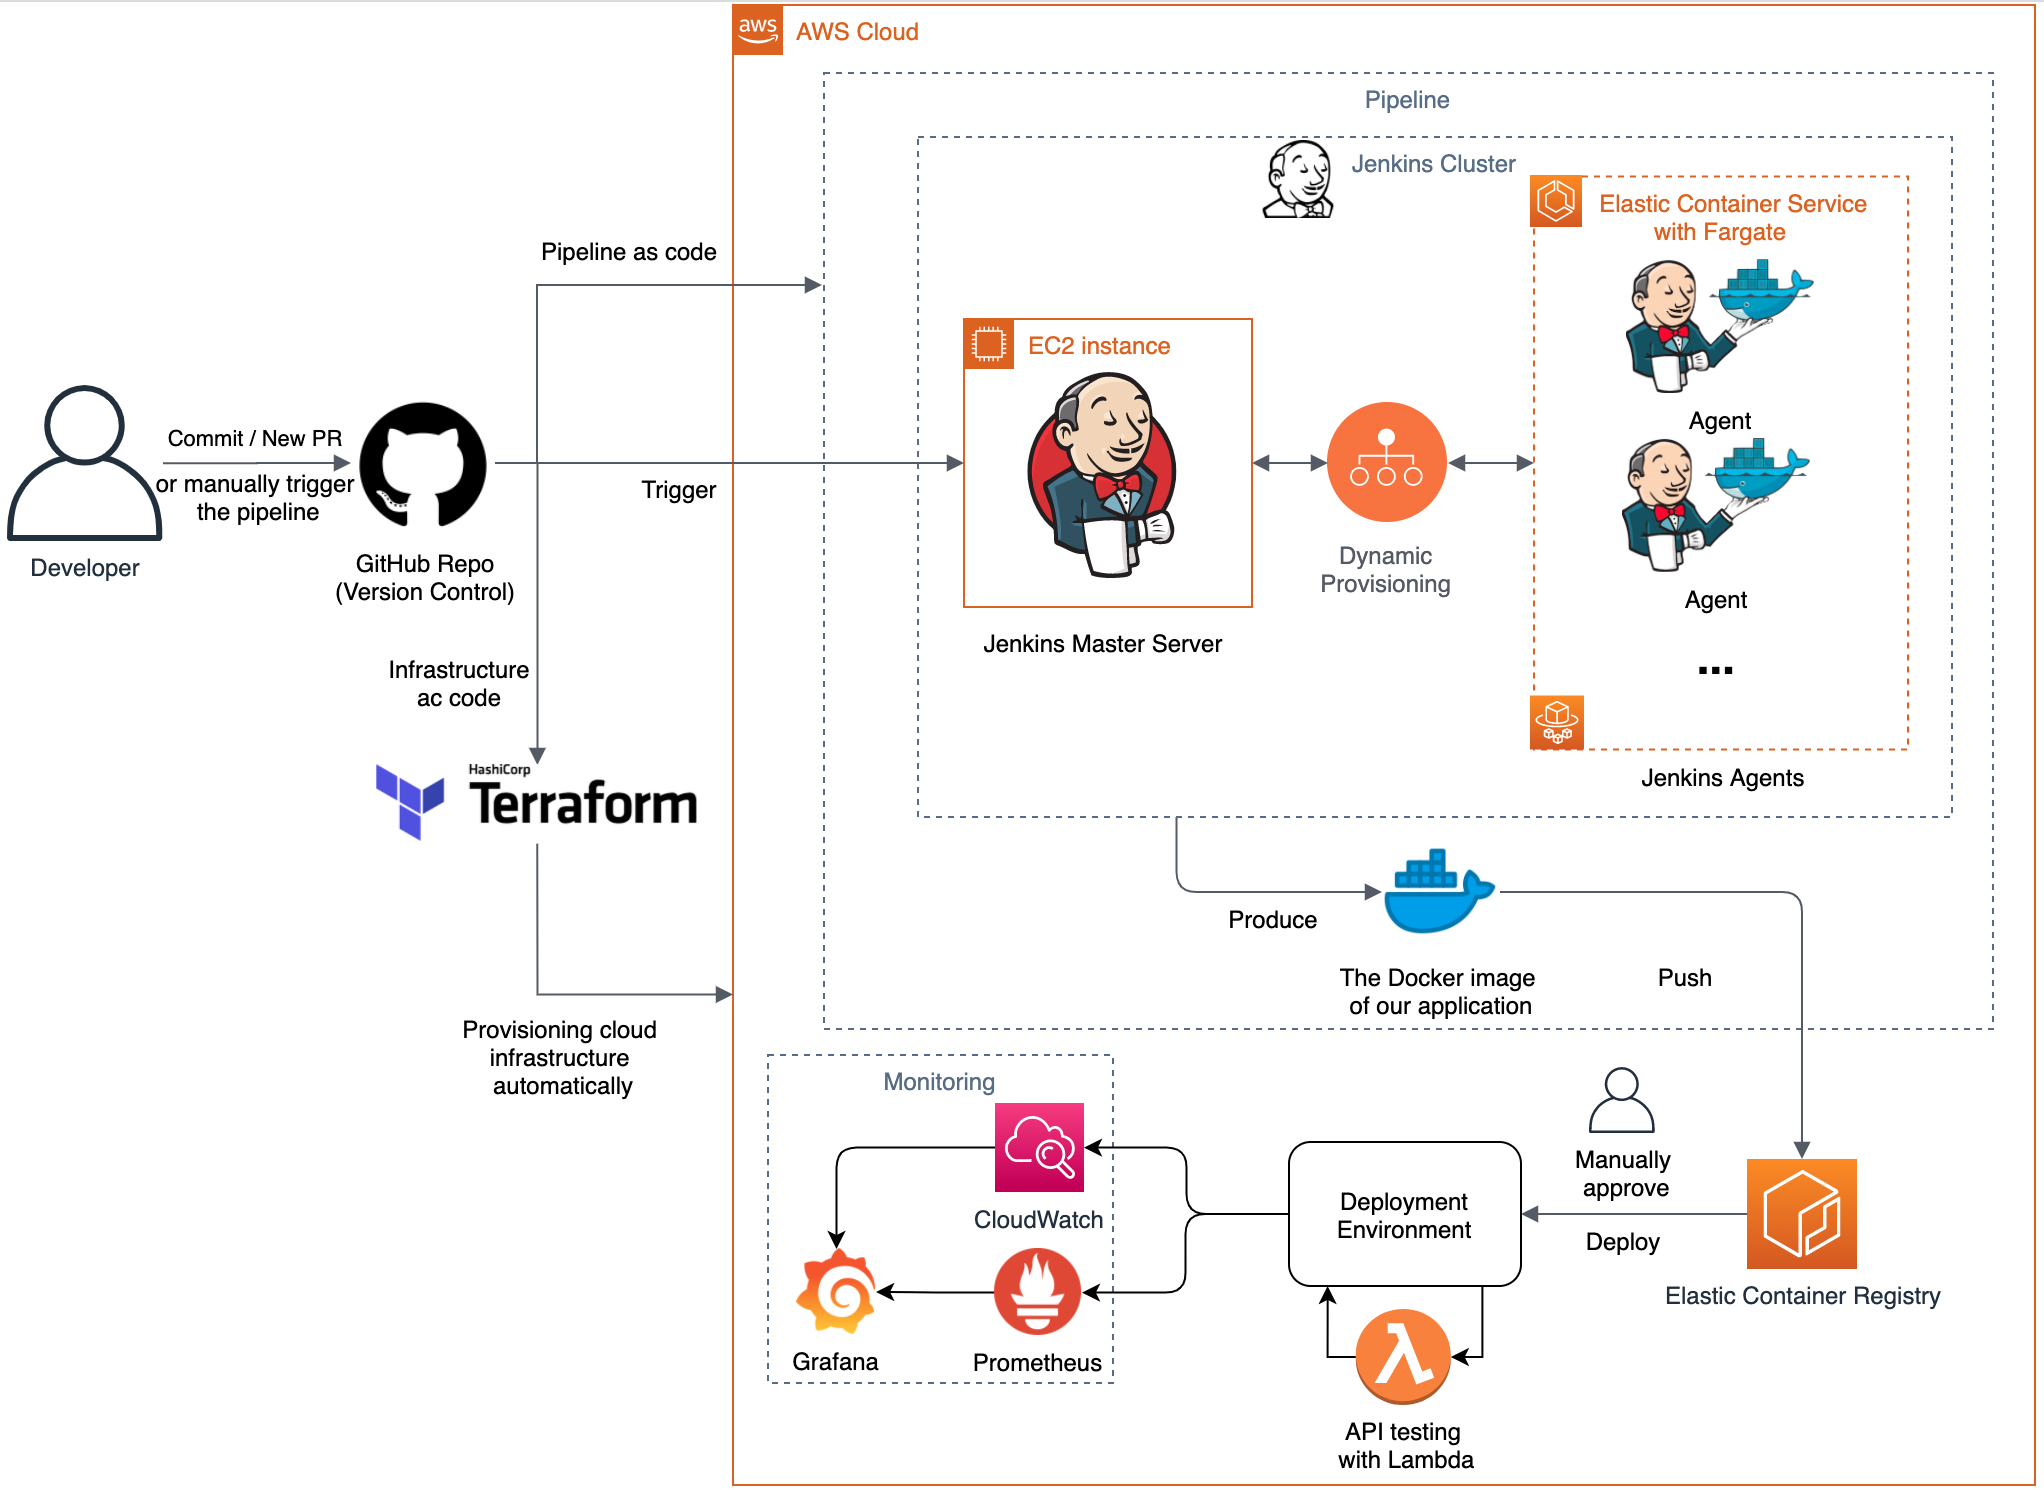
\includegraphics[width=0.99\textwidth]{pics/arch-med-jenkins.png}
    \caption{Architecture diagram of our DevOps toolchain}
    \label{fig:archjenkins}
\end{figure}
The toolchain implementation is based on the DevOps elements we presented in Chapter 2, and the DevOps practises from Eficode. Figure \ref{fig:archjenkins} shows the architecture of our DevOps toolchain. In here we only presenting architecture on a more general level. The detailed architecture of each component will be introduced in the following sections, in both text and graph.
\par
When the developer pushes a new commit to the repository in GitHub \footnote{https://github.com/}, Github will send an HTTP POST request that contains the necessary information to the Jenkins master node. Jenkins master which triggered by the HTTP request will create a new job for this project according to the information that the HTTP request contains. The job will first pull the latest code from the git repository, then runs the docker containers with required build environment and build the project. In the end, a docker image for running the project will be created and be pushed to the container registry of AWS. Depends on the git branch that the developer committed to, the project will be deployed to a different development environment.
\par
Figure \ref{fig:archjenkins} shows the architecture of our DevOps toolchain. We can see except version control, the whole environment is running in Amazon Web Services. Due to the limitation of space, the internal architecture of certain components is not shown in the graph, instead, we show them in the following sections.
\subsection{Version Control}
Version Control System (VCS) is the process that record the changes in files set over time \cite{GitAbout93:online}, and versioning the history of these files. VSC is suitable for track the development progress and manages the goal within a software development team \cite{loeliger2012version}. Among all software for version control, Git is the most popular one nowadays. The survey \cite{CompareR31:online} from Synopsys shows that in 2019, 71\% of the project today is using Git as it's versioning system while SVN that ranks in second only be used in 25\% of the projects. We use Git as the version control system since it is used by most of the software development teams nowadays. We use GitHub for hosting the case project. Github is the biggest preform in the world that hosting a version-controlled software project for free using Git. It provides interfaces with different DevOps related tools which makes it easy to be integrated into all kinds of DevOps toolchains.
\begin{figure}[h]
    \centering
    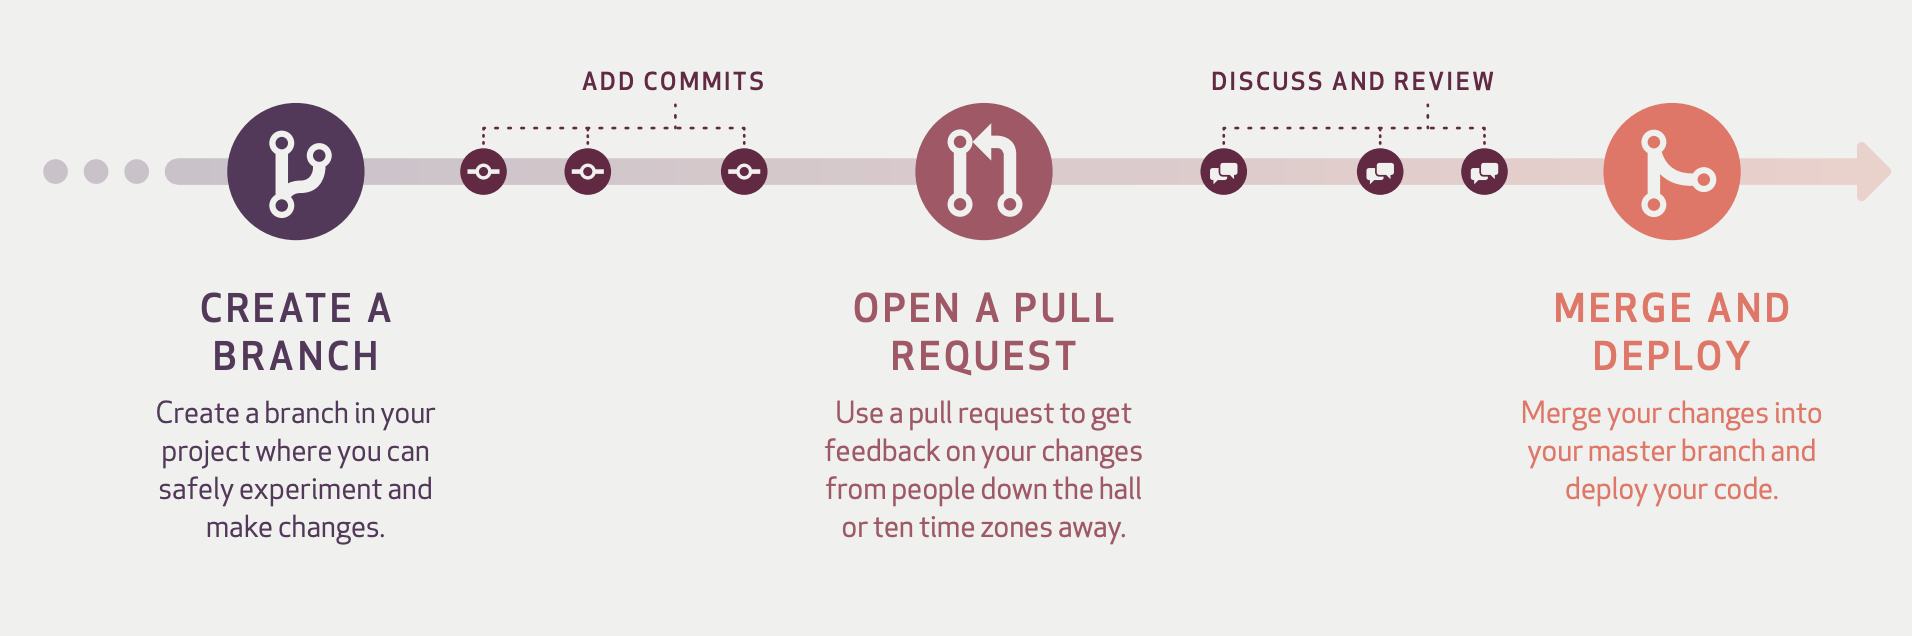
\includegraphics[width=0.99\textwidth]{pics/git.png}
    \caption{GitHub Workflow \cite{guides2013understanding}}
    \label{fig:git}
\end{figure}
\par
The Git flow \cite{driessen2010successful} proposed in 2010 is a successful workflow for working with Git. Git flow has already widely used and has been approved by the software industries. However, to better cope with the frequent release nature of DevOps, the Github workflow -- a simplified version of Git flow is proposed by GitHub.
Therefore GitHub workflow \cite{chacongithub} is being chosen as our workflow in the version control. The simplified version of this workflow is shown as in Figure \ref{fig:git}
\par
Several general principals followed by us when adapting GitHub flow, we refer the principals in \cite{chacongithub} to design our workflow.
\begin{itemize}
    \item Master branch is always deployable. This means when deploying the continuous delivery pipelines in our toolchain, only the master branch can be deployed. And there shouldn't have any code which is not good to be deployed in the master branch. 
    \item When working on the new feature, make a new branch for this feature. The name of this branch should be descriptive which reflect the content of this feature. Commit the code related to this feature this branch and push from this branch to the branch with the same name on the remote server (github.com).
    \item Open a pull request\footnote{https://help.github.com/en/GitHub/collaborating-with-issues-and-pull-requests/about-pull-requests} when the feature is ready to merge, or when you feel that you need help or comments from other team means on this feature. The code review is also done by others in the pull request.
    \item When the code is already be reviewed and is good to be merged, the developer should merge the code to the master.
    \item After the code of this feature is in the master, the code will and should be immediately deployed. There should not be any rollback in the master branch. If there are any issues within the newly merged code, a new commit or a new branch should be made to fix the issue rather than rollback on the master.
\end{itemize}
\par
Note that in our Git workflow, there are several time points that we need to run the continuous delivery pipeline within the toolchain. The continuous delivery pipeline will also vary with the time point within the version control workflow. We will introduce this in detail on \ref{our-ci}.
\subsection{Continuous Delivery Pipeline}
\label{our-ci}
\subsubsection{Tool Selection Considerations}
The most popular server-based tools for build continuous delivery pipeline are Jenkins\footnote{https://www.jenkins.io/}, Drone\footnote{https://drone.io/}, GoCD\footnote{https://www.gocd.org/} and Circle CI\footnote{https://circleci.com/}. A comparison between these tools is shown in Table \ref{tab:ci-tools}. As we can see from the table, Jenkins is the most popular option for CI/CD. Jenkins has wide application in the commercial use case, and the high popularity in the open-source community as well. Although compared with the other 3 newer tools, Jenkins is more focuses on the "Build" step within the continuous delivery pipeline. However, the open-source nature of Jenkins gives it a much wider selection of the plugin, which males Jenkins can be used for almost all steps in a continuous delivery pipeline. 
\begin{table}[h]
    \begin{tabular}{|l|l|l|l|l|}
    \hline
                        & Jenkins & Drone & Circle CI & GoCD \\ \hline
    Open Source         & Yes     & Yes   & No        & Yes  \\ \hline
    GitHub stars        & 15.7k   & 21.2k & -         & 5.7k \\ \hline
    Github contributors & 614     & 258   & -         & 116  \\ \hline
    Plugin extensions &
      Over 1500 \tablefootnote{https://plugins.jenkins.io/} &
      93 \tablefootnote{According to GitHub search result} &
      110 \tablefootnote{https://circleci.com/integrations/} &
      88 \tablefootnote{https://www.gocd.org/plugins/} \\ \hline
    \begin{tabular}[c]{@{}l@{}}Price of self-hosted \\ solution\end{tabular} &
      Free &
      Free &
      \$35 user/month &
      Free \\ \hline
    \begin{tabular}[c]{@{}l@{}}Number of companies\\use it in the tech stack\tablefootnote{based on data from StackShare}\end{tabular} &
      2634 &
      82 &
      1368 &
      42 \\ \hline
    \end{tabular}
    \caption{Comparison of continuous delivery tools}
    \label{tab:ci-tools}
    \end{table}
\par
Created by Kohsuke Kawaguchi in 2001, Jenkins is an open-source continuous integrating tool write with Java.  It is suitable for a team of all sizes and varies of languages and technologies \cite{smart2011jenkins}. Furthermore, Jenkins also attracts software teams with it's easy-to-use and high extendibility \cite{smart2011jenkins} with thousand of the plugin. More plugin keeps coming since Jenkins has an active open-source community. These plugins help Jenkins keep up with the fast-developing DevOps practices, and help Jenkins integrate with the newly emerging tools and cloud services. The extendibility makes Jenkins still the most popular tool for DevOps toolchain even it's an aged software created when the term "DevOps" just appeared.
\par
Our continuous delivery pipeline is built with Pipeline plugin\footnote{https://www.jenkins.io/doc/book/pipeline/} in Jenkins. 
Pipeline plugin allows us to define a continuous delivery pipeline as code in Jenkinsfile.
In the pipeline, a conceptually distinct subset of tasks within the continuous delivery pipeline \cite{Pipeline85:online} is defined as a "stage"\footnote{For example, "Build", Test", "Deploy" step in a continuous delivery pipeline.} and each task within a step is called "step". Each pipeline is binding with a "project". An execution runtime of a project/pipeline is called "build" and the machine (virtual machine, container, etc.) for running the build is called "agent".
\par
Figure \ref{fig:pipeline} shows the workflow of a project going through our continuous delivery pipeline. The developer only commit to the feature branch. The pipeline runs after developer push local commits to Git. When the pipeline is triggered by the event on the feature branch, it only runs the first half. 
\begin{figure}[h]
    \centering
    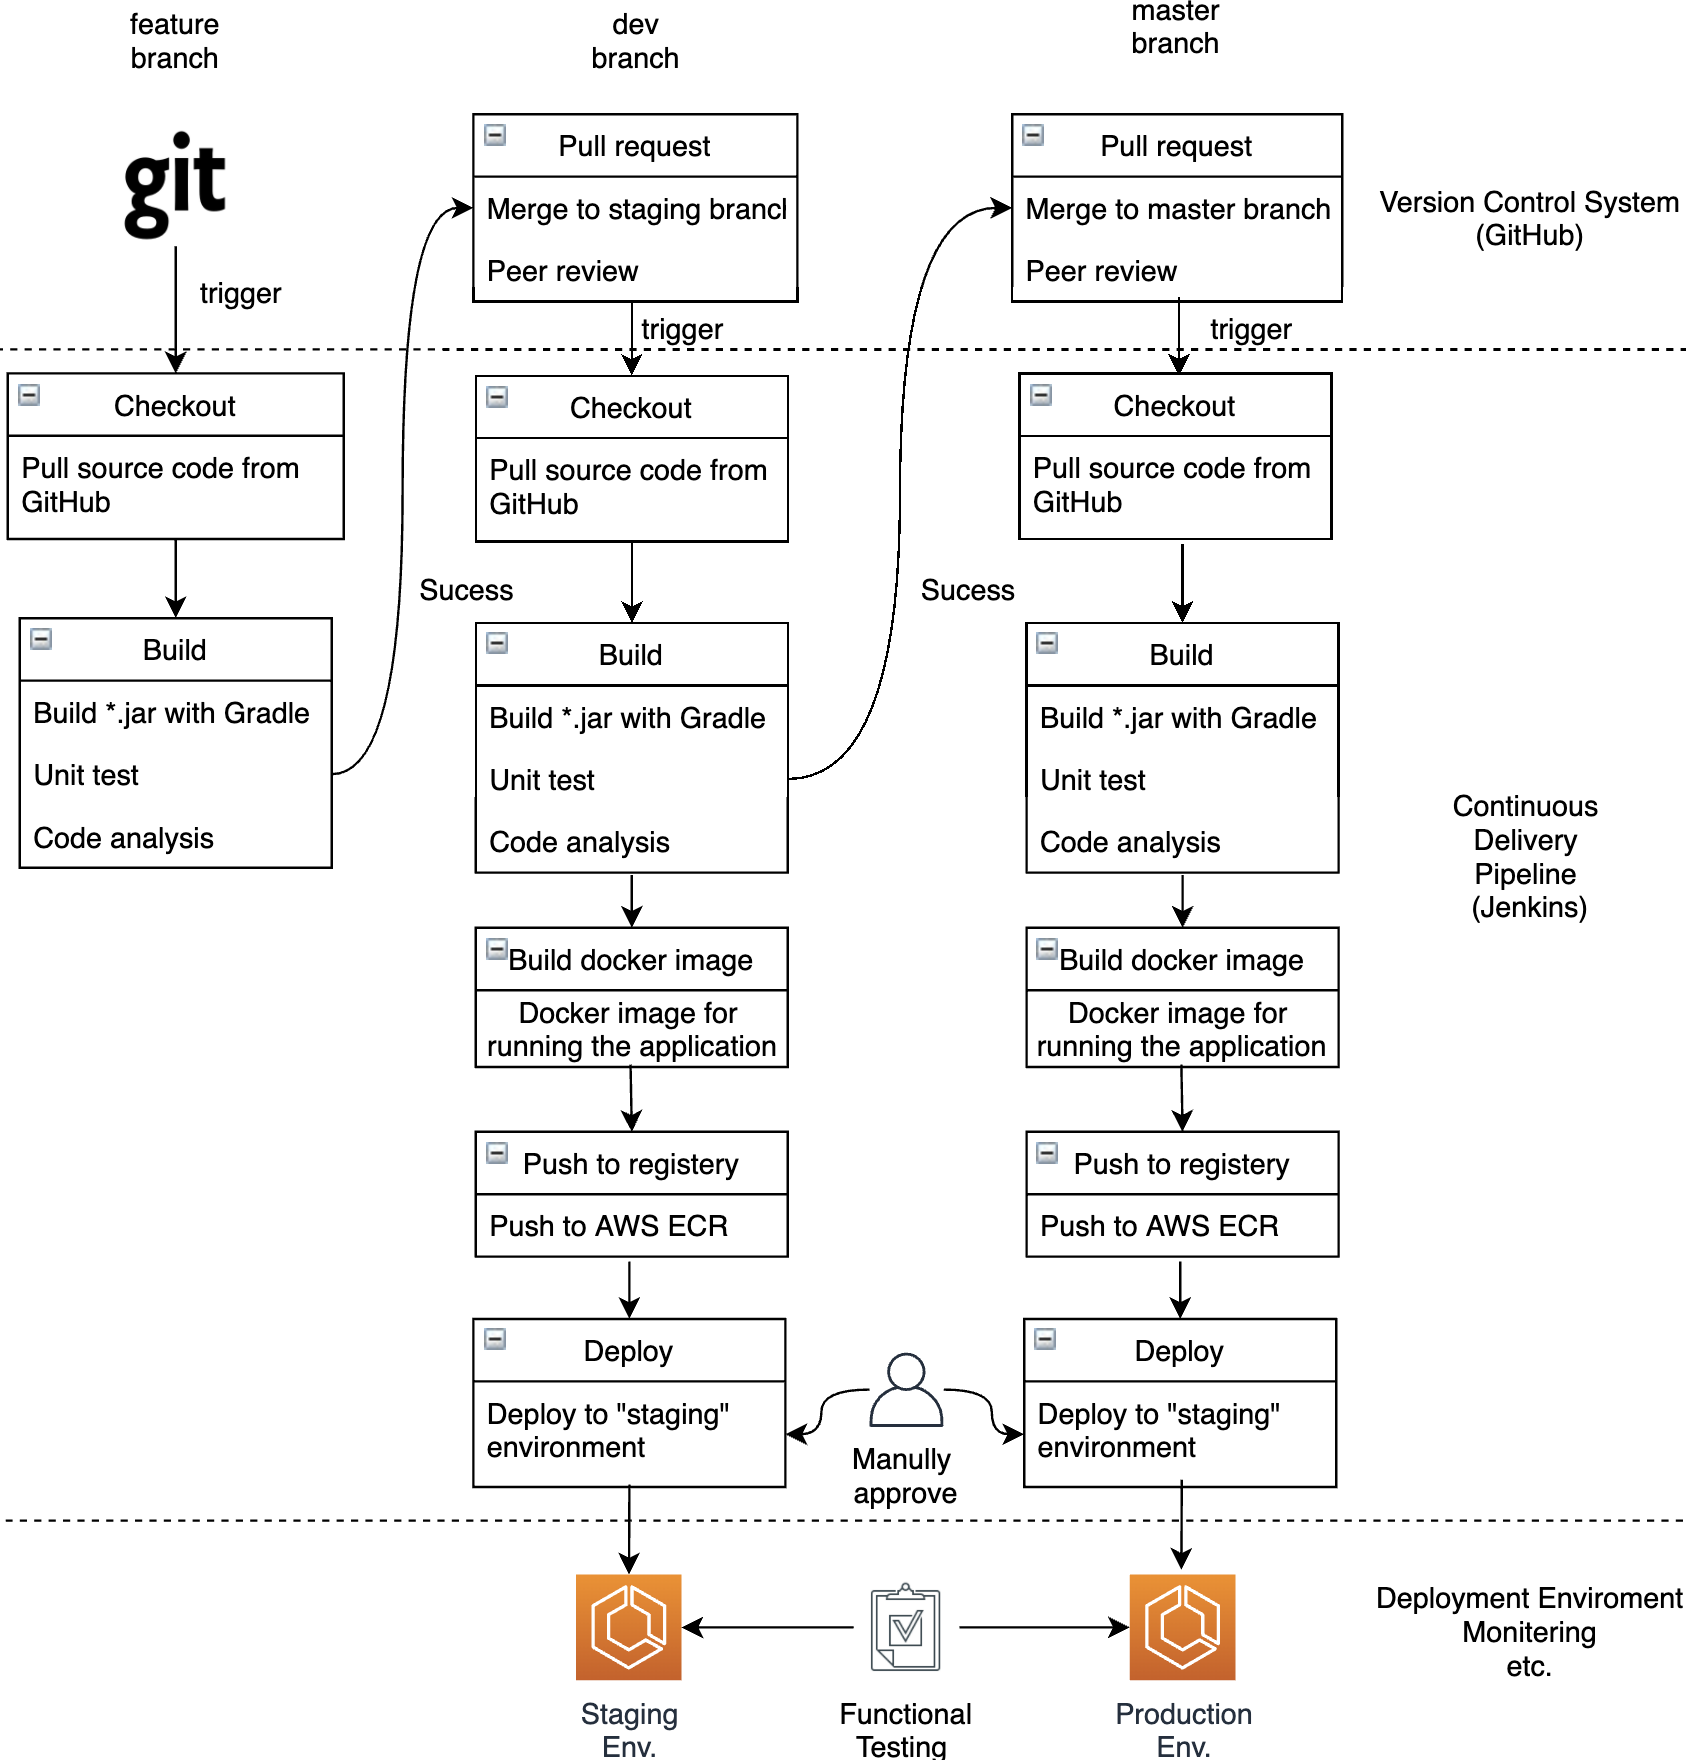
\includegraphics[width=0.99\textwidth]{pics/pipeline.png}
    \caption{Continuous Delivery Pipeline in Our DevOps Toolchain}
    \label{fig:pipeline}
\end{figure}

\subsubsection{Deployment}
We using Martin Fowler's blue and green deployment strategy \cite{fowler2010bluegreendeployment}
\subsection{Monitoring}
\section{Design of Serverless DevOps Toolchain}
% \section{Cloud Services}
% \label{assumption}
% In this section, we will introduce several could service from CH3 that could be helpful to the DevOps toolchain. 
% //  Using services in AWS as an example, Introduces how cloud services could improve. describe services in one section
% \subsection{Managed Container Services for Distributed Builds} 

% // Describe how AWS Fargate could Help
% \subsection{Serverless computing}
% // Describe how AWS lambda could Help and why do we chose it
% \subsection{...}
